\documentclass[14pt]{extarticle}
% math symbols
\usepackage{sfg}


\usepackage{amssymb,amsmath}
\synctex=1
% for different compilers
\usepackage{ifpdf}
% geometry of page
\usepackage[margin=2cm]{geometry}

% if pdflatex, then
\ifpdf
\usepackage[russian]{babel}
\usepackage[utf8]{inputenc}
\usepackage[unicode]{hyperref}
\usepackage[pdftex]{graphicx}
\usepackage{cmlgc}
% if xelatex, then
\else
% math fonts
\usepackage{fouriernc}
% xelatex specific packages
\usepackage[xetex]{hyperref}
\usepackage{xltxtra}	% \XeLaTeX macro
\usepackage{xunicode}	% some extra unicode support
\defaultfontfeatures{Mapping=tex-text}
\usepackage{polyglossia}	% instead of babel in xelatex
\usepackage{indentfirst}	% 
\setdefaultlanguage{russian}
% fonts
\newfontfamily\cyrillicfont{SchoolBookC}
\newfontfamily\cyrillicfontsf{TextBookC}
\setmonofont{Consolas}
\fi

% several pictures in one figure
\usepackage{subfig}
% calc in TeX expressions
\usepackage{calc}
% nice pictures and plots
\usepackage{pgfplots,tikz,circuitikz}
% different libraries for pictures
\usetikzlibrary{%
  arrows,%
  calc,%
  patterns,%
  decorations.pathreplacing,%
  decorations.pathmorphing,%
  decorations.markings,%
  intersections,%
  decorations.text%
}

\usepackage{tkz-euclide}

\usepackage{enumitem}
\renewcommand{\theenumi}{(\asbuk{enumi})}
\renewcommand{\labelenumi}{\asbuk{enumi})}
\AddEnumerateCounter{\Asbuk}{\@Asbuk}{\CYRM}
\AddEnumerateCounter{\asbuk}{\@asbuk}{\cyrm}

\begin{document}

\section*{Задача}

\subsection*{Условие}
Нарисуйте двa треугольника $ABC$ и $CBD$, не лежащих в одной плоскости. Внутри отрезков $AD$ и $BD$ возьмите точки $K$ и $L$.

\begin{enumerate}

\item Пусть $(KL)$ пересекает $(AB)$ в точке $M$. Объясните, почему точка M является точкой пересечения $(KL)$и $(ABC)$.
\item Пусть $(KL)$и $(AB)$не пересекаются. Объясните, почему в этом случае $(KL)$и $(ABC)$ не пересекаются.

\end{enumerate}
\subsection*{Решение}
\begin{enumerate}
\item Точка $M\in (AB)$, $(AB)\subset ABC \Rightarrow M\in ABC$. Также $M\in KL$. А Значит точка M является точкой пересечения $(KL)$ и $(ABC)$.
\item Допустим $(KL)$ и $ABC$ пересекаются в точке $M$. Тогда $M\in (AB)$. Противоречие.
\end{enumerate}
\newpage
\begin{figure}[h]
	\centering
	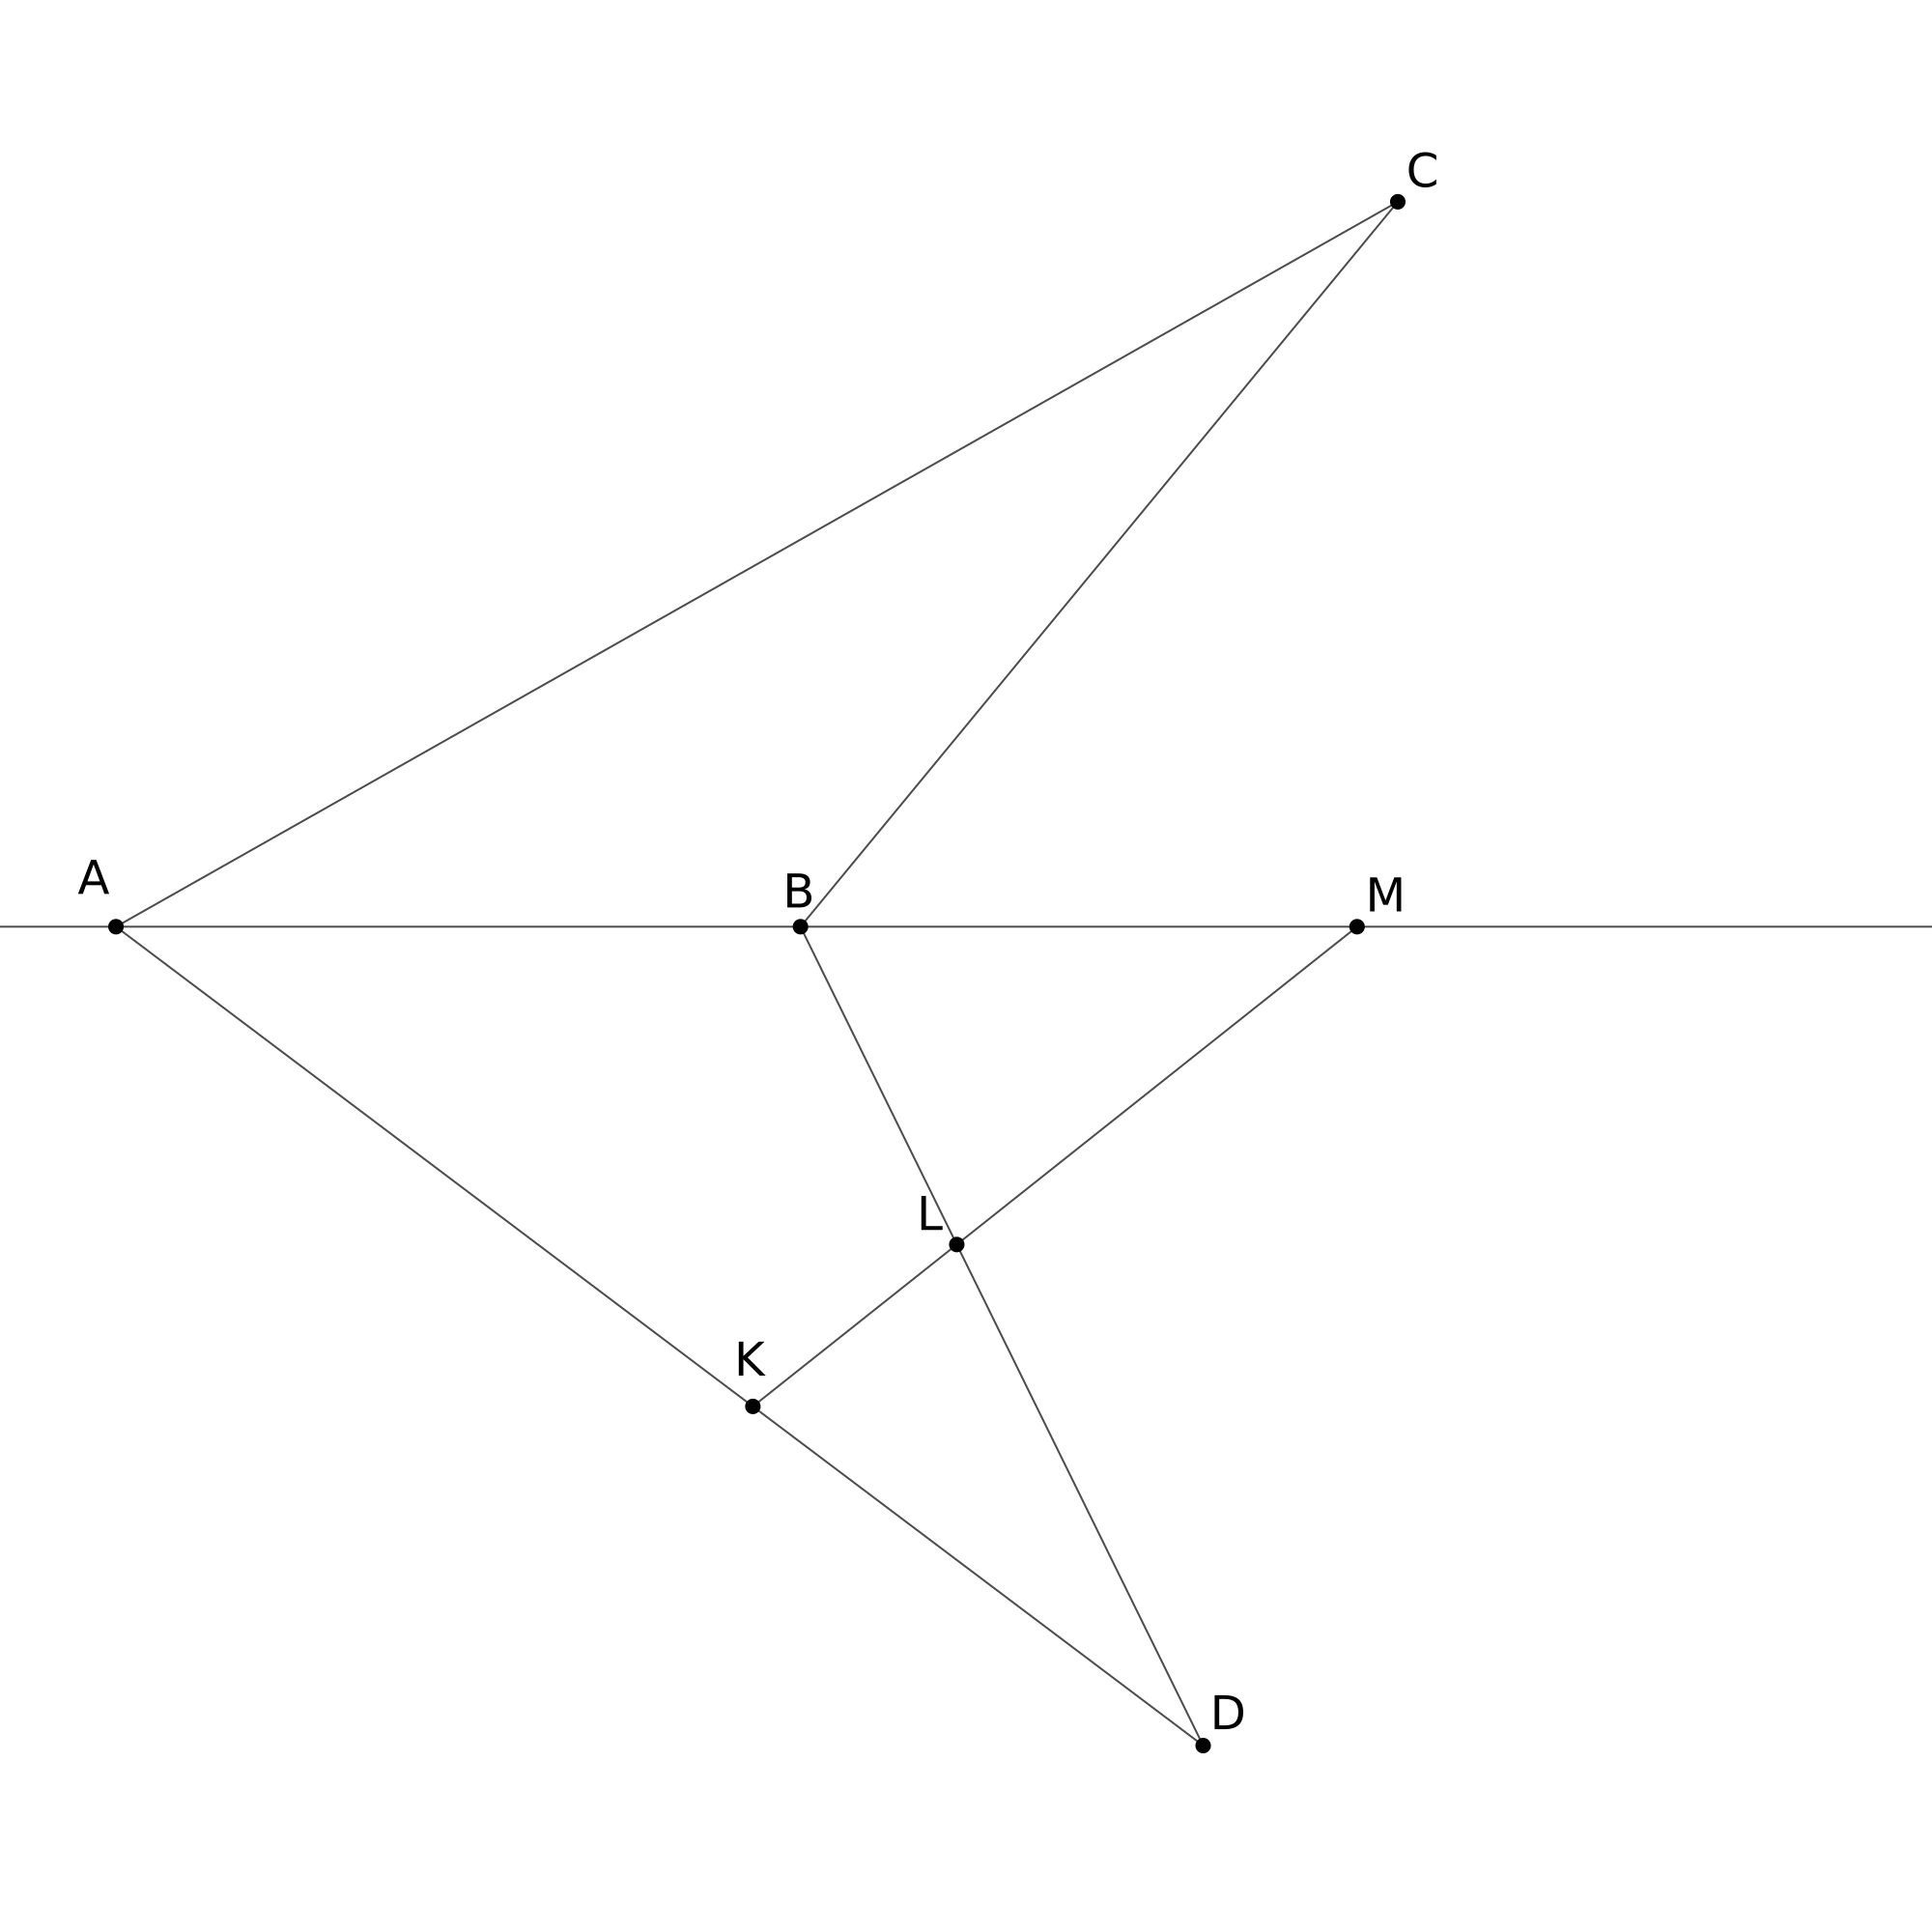
\includegraphics[width=1\textwidth]{{/home/galqiwi/geoma/2.3}.png}
\end{figure}


\end{document}